
\begin{TP}[Le puzzle qui s'agrandit]

\partie{Création d'un modèle}
\begin{minipage}[c]{0.48\linewidth}
\begin{enumerate}
 \item Tracez un carré de 5 cm de côté pour le groupe. Partagez-le en autant de pièces (triangles rectangles, carrés, rectangles, trapèzes \ldots) que de membres du groupe.
 
Vous obtenez un puzzle du carré.
 \item Déterminez ensemble les dimensions de chaque pièce.
 \end{enumerate}
\end{minipage} \hfill%
 \begin{minipage}[c]{0.4\linewidth}
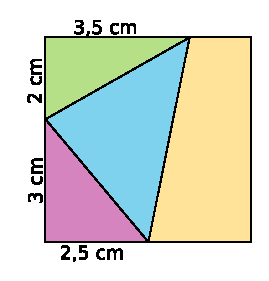
\includegraphics[width=4cm]{carre_puzzle}
 \end{minipage} \\

\partie{Agrandissement}
On souhaite agrandir le puzzle. \\[0.5em]
Chaque élève du groupe choisit une pièce et la reproduit avec de nouvelles dimensions de façon à ce que le puzzle reconstitué soit un carré de 12 cm de côté.

\partie{Vérification}
Vérifiez en essayant de reconstituer le puzzle.

\end{TP}

